\documentclass[a4paper]{book}
\usepackage{a4wide}
\usepackage{makeidx}
\usepackage{graphicx}
\usepackage{multicol}
\usepackage{float}
\usepackage{listings}
\usepackage{color}
\usepackage{textcomp}
\usepackage{alltt}
\usepackage{times}
\usepackage{ifpdf}
\ifpdf
\usepackage[pdftex,
            pagebackref=true,
            colorlinks=true,
            linkcolor=blue,
            unicode
           ]{hyperref}
\else
\usepackage[ps2pdf,
            pagebackref=true,
            colorlinks=true,
            linkcolor=blue,
            unicode
           ]{hyperref}
\usepackage{pspicture}
\fi
\usepackage[utf8]{inputenc}
\usepackage{doxygen}
\lstset{language=C++,inputencoding=utf8,basicstyle=\footnotesize,breaklines=true,breakatwhitespace=true,tabsize=8,numbers=left }
\makeindex
\setcounter{tocdepth}{3}
\renewcommand{\footrulewidth}{0.4pt}
\begin{document}
\hypersetup{pageanchor=false}
\begin{titlepage}
\vspace*{7cm}
\begin{center}
{\Large KeyValueClusterPerf }\\
\vspace*{1cm}
{\large Generated by Doxygen 1.6.1}\\
\vspace*{0.5cm}
{\small Mon Aug 10 15:03:41 2015}\\
\end{center}
\end{titlepage}
\clearemptydoublepage
\pagenumbering{roman}
\tableofcontents
\clearemptydoublepage
\pagenumbering{arabic}
\hypersetup{pageanchor=true}
\chapter{Data Structure Index}
\section{Class Hierarchy}
This inheritance list is sorted roughly, but not completely, alphabetically:\begin{DoxyCompactList}
\item \contentsline{section}{AccessPattern}{\pageref{classAccessPattern}}{}
\begin{DoxyCompactList}
\item \contentsline{section}{RandomAccessPattern}{\pageref{classRandomAccessPattern}}{}
\item \contentsline{section}{ReadOnlyAccessPattern}{\pageref{classReadOnlyAccessPattern}}{}
\end{DoxyCompactList}
\item \contentsline{section}{ConfigurationManager}{\pageref{classConfigurationManager}}{}
\item \contentsline{section}{KeyValueDB}{\pageref{classKeyValueDB}}{}
\begin{DoxyCompactList}
\item \contentsline{section}{DummyKeyValueDB}{\pageref{classDummyKeyValueDB}}{}
\item \contentsline{section}{RamCloudKeyValueDB}{\pageref{classRamCloudKeyValueDB}}{}
\item \contentsline{section}{RiakCKeyValueDB}{\pageref{classRiakCKeyValueDB}}{}
\item \contentsline{section}{RiakJavaKeyValueDB}{\pageref{classRiakJavaKeyValueDB}}{}
\end{DoxyCompactList}
\item \contentsline{section}{MessageSender}{\pageref{classMessageSender}}{}
\item \contentsline{section}{messaging::RequestMessage}{\pageref{classmessaging_1_1RequestMessage}}{}
\item \contentsline{section}{SimulationController}{\pageref{classSimulationController}}{}
\item \contentsline{section}{SimulationWorker}{\pageref{classSimulationWorker}}{}
\item \contentsline{section}{Simulator}{\pageref{classSimulator}}{}
\item \contentsline{section}{SingleAccess}{\pageref{structSingleAccess}}{}
\item \contentsline{section}{messaging::StaticDescriptorInitializer\_\-request\_\-2eproto}{\pageref{structmessaging_1_1StaticDescriptorInitializer__request__2eproto}}{}
\item \contentsline{section}{ValueDistribution}{\pageref{classValueDistribution}}{}
\begin{DoxyCompactList}
\item \contentsline{section}{ConstantValueDistribution}{\pageref{classConstantValueDistribution}}{}
\end{DoxyCompactList}
\end{DoxyCompactList}

\chapter{Data Structure Index}
\section{Data Structures}
Here are the data structures with brief descriptions:\begin{DoxyCompactList}
\item\contentsline{section}{\hyperlink{classAccessPattern}{AccessPattern} }{\pageref{classAccessPattern}}{}
\item\contentsline{section}{\hyperlink{classConfigurationManager}{ConfigurationManager} }{\pageref{classConfigurationManager}}{}
\item\contentsline{section}{\hyperlink{classConstantValueDistribution}{ConstantValueDistribution} }{\pageref{classConstantValueDistribution}}{}
\item\contentsline{section}{\hyperlink{classDummyKeyValueDB}{DummyKeyValueDB} }{\pageref{classDummyKeyValueDB}}{}
\item\contentsline{section}{\hyperlink{classKeyValueDB}{KeyValueDB} }{\pageref{classKeyValueDB}}{}
\item\contentsline{section}{\hyperlink{classMessageSender}{MessageSender} }{\pageref{classMessageSender}}{}
\item\contentsline{section}{\hyperlink{classRamCloudKeyValueDB}{RamCloudKeyValueDB} }{\pageref{classRamCloudKeyValueDB}}{}
\item\contentsline{section}{\hyperlink{classRandomAccessPattern}{RandomAccessPattern} }{\pageref{classRandomAccessPattern}}{}
\item\contentsline{section}{\hyperlink{classReadOnlyAccessPattern}{ReadOnlyAccessPattern} }{\pageref{classReadOnlyAccessPattern}}{}
\item\contentsline{section}{\hyperlink{classmessaging_1_1RequestMessage}{messaging::RequestMessage} }{\pageref{classmessaging_1_1RequestMessage}}{}
\item\contentsline{section}{\hyperlink{classRiakCKeyValueDB}{RiakCKeyValueDB} }{\pageref{classRiakCKeyValueDB}}{}
\item\contentsline{section}{\hyperlink{classRiakJavaKeyValueDB}{RiakJavaKeyValueDB} }{\pageref{classRiakJavaKeyValueDB}}{}
\item\contentsline{section}{\hyperlink{classSimulationController}{SimulationController} }{\pageref{classSimulationController}}{}
\item\contentsline{section}{\hyperlink{classSimulationWorker}{SimulationWorker} }{\pageref{classSimulationWorker}}{}
\item\contentsline{section}{\hyperlink{classSimulator}{Simulator} }{\pageref{classSimulator}}{}
\item\contentsline{section}{\hyperlink{structSingleAccess}{SingleAccess} }{\pageref{structSingleAccess}}{}
\item\contentsline{section}{\hyperlink{structmessaging_1_1StaticDescriptorInitializer__request__2eproto}{messaging::StaticDescriptorInitializer\_\-request\_\-2eproto} }{\pageref{structmessaging_1_1StaticDescriptorInitializer__request__2eproto}}{}
\item\contentsline{section}{\hyperlink{classValueDistribution}{ValueDistribution} }{\pageref{classValueDistribution}}{}
\end{DoxyCompactList}

\chapter{Data Structure Documentation}
\hypertarget{classAccessPattern}{
\section{AccessPattern Class Reference}
\label{classAccessPattern}\index{AccessPattern@{AccessPattern}}
}


{\ttfamily \#include $<$AccessPattern.h$>$}Inheritance diagram for AccessPattern::\begin{figure}[H]
\begin{center}
\leavevmode
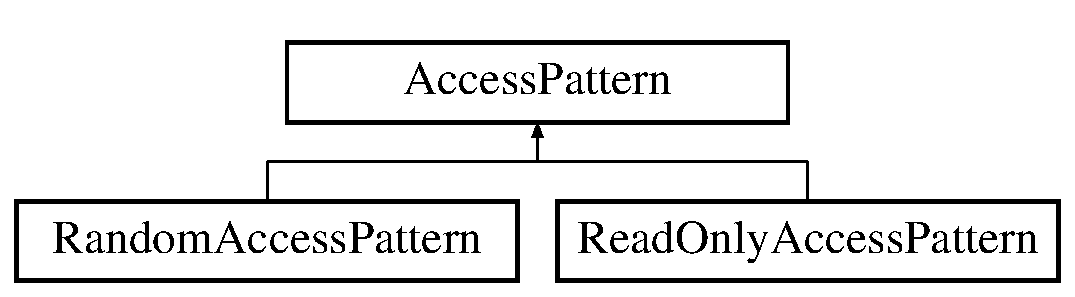
\includegraphics[height=2cm]{classAccessPattern}
\end{center}
\end{figure}
\subsection*{Public Member Functions}
\begin{DoxyCompactItemize}
\item 
virtual \hyperlink{structSingleAccess}{SingleAccess} \hyperlink{classAccessPattern_a8c46aedb717e862598524f250f23086f}{getNext} ()=0
\item 
virtual map$<$ string, string $>$ \hyperlink{classAccessPattern_afa72bed11401bfd96e8fa88acd72934b}{getInitialisationKeyValuePairs} ()=0
\item 
void \hyperlink{classAccessPattern_a80227f44091a53a2798b44e4e54f3484}{setValueDistribution} (\hyperlink{classValueDistribution}{ValueDistribution} $\ast$valueDistribution)
\end{DoxyCompactItemize}
\subsection*{Protected Attributes}
\begin{DoxyCompactItemize}
\item 
\hypertarget{classAccessPattern_af87b840d2a9edad3c3fbf9a521844588}{
\hyperlink{classValueDistribution}{ValueDistribution} $\ast$ {\bfseries valueDistribution}}
\label{classAccessPattern_af87b840d2a9edad3c3fbf9a521844588}

\end{DoxyCompactItemize}


\subsection{Detailed Description}
Abstract class \hyperlink{classAccessPattern}{AccessPattern} represents a set of functions to be implemented by each accessPattern This class defines the accesses to the database and generates \hyperlink{structSingleAccess}{SingleAccess} returns 

\subsection{Member Function Documentation}
\hypertarget{classAccessPattern_afa72bed11401bfd96e8fa88acd72934b}{
\index{AccessPattern@{AccessPattern}!getInitialisationKeyValuePairs@{getInitialisationKeyValuePairs}}
\index{getInitialisationKeyValuePairs@{getInitialisationKeyValuePairs}!AccessPattern@{AccessPattern}}
\subsubsection[{getInitialisationKeyValuePairs}]{\setlength{\rightskip}{0pt plus 5cm}virtual map$<$string,string$>$ AccessPattern::getInitialisationKeyValuePairs ()\hspace{0.3cm}{\ttfamily  \mbox{[}pure virtual\mbox{]}}}}
\label{classAccessPattern_afa72bed11401bfd96e8fa88acd72934b}
get key-\/value pairs to initialise database before simulation. This prevents access to non-\/existend items 

Implemented in \hyperlink{classRandomAccessPattern_a72da825a9cb74f58fcadf6fc894d5e82}{RandomAccessPattern}, and \hyperlink{classReadOnlyAccessPattern_a2e6ce8d90050b038ffbf643b344e0eb5}{ReadOnlyAccessPattern}.\hypertarget{classAccessPattern_a8c46aedb717e862598524f250f23086f}{
\index{AccessPattern@{AccessPattern}!getNext@{getNext}}
\index{getNext@{getNext}!AccessPattern@{AccessPattern}}
\subsubsection[{getNext}]{\setlength{\rightskip}{0pt plus 5cm}virtual {\bf SingleAccess} AccessPattern::getNext ()\hspace{0.3cm}{\ttfamily  \mbox{[}pure virtual\mbox{]}}}}
\label{classAccessPattern_a8c46aedb717e862598524f250f23086f}
generate the next access information to the database 

Implemented in \hyperlink{classRandomAccessPattern_a5b590afc37a8bf5e4a4235834c6ebe12}{RandomAccessPattern}, and \hyperlink{classReadOnlyAccessPattern_a324b6da6296a17144d51db2841e16ba4}{ReadOnlyAccessPattern}.\hypertarget{classAccessPattern_a80227f44091a53a2798b44e4e54f3484}{
\index{AccessPattern@{AccessPattern}!setValueDistribution@{setValueDistribution}}
\index{setValueDistribution@{setValueDistribution}!AccessPattern@{AccessPattern}}
\subsubsection[{setValueDistribution}]{\setlength{\rightskip}{0pt plus 5cm}void AccessPattern::setValueDistribution ({\bf ValueDistribution} $\ast$ {\em valueDistribution})}}
\label{classAccessPattern_a80227f44091a53a2798b44e4e54f3484}
Assign the accessPattern class which valueDistribution to use during generation of the next access 

The documentation for this class was generated from the following files:\begin{DoxyCompactItemize}
\item 
src/AccessPattern.h\item 
src/AccessPattern.cc\end{DoxyCompactItemize}

\hypertarget{classConfigurationManager}{
\section{ConfigurationManager Class Reference}
\label{classConfigurationManager}\index{ConfigurationManager@{ConfigurationManager}}
}


{\ttfamily \#include $<$ConfigurationManager.h$>$}\subsection*{Public Member Functions}
\begin{DoxyCompactItemize}
\item 
map$<$ string, string $>$ \hyperlink{classConfigurationManager_a1c4ee8379e2ccee2a2ac76b92042daba}{readFile} (string fileName)
\item 
void \hyperlink{classConfigurationManager_a078649c42cbc46e6fbdf7b7a74183898}{writeFile} (string fileName, map$<$ string, string $>$ configuration)
\item 
map$<$ string, string $>$ \hyperlink{classConfigurationManager_aed48081116dc9181acb904ac18a52eb5}{readString} (string str)
\item 
string \hyperlink{classConfigurationManager_a4dfba4665ffb818e21363f446a6cde12}{writeString} (map$<$ string, string $>$ configuration)
\item 
list$<$ string $>$ \hyperlink{classConfigurationManager_adba6ce19eaf7b98ba158011f4bb71eea}{readHostFile} (string fileName)
\end{DoxyCompactItemize}


\subsection{Detailed Description}
\hyperlink{classConfigurationManager}{ConfigurationManager} contains all functionality to read and write configuration files used in \hyperlink{classAccessPattern}{AccessPattern}, \hyperlink{classKeyValueDB}{KeyValueDB} and \hyperlink{classValueDistribution}{ValueDistribution} as well as reading in the hostfile in \hyperlink{classSimulationController}{SimulationController} 

\subsection{Member Function Documentation}
\hypertarget{classConfigurationManager_a1c4ee8379e2ccee2a2ac76b92042daba}{
\index{ConfigurationManager@{ConfigurationManager}!readFile@{readFile}}
\index{readFile@{readFile}!ConfigurationManager@{ConfigurationManager}}
\subsubsection[{readFile}]{\setlength{\rightskip}{0pt plus 5cm}map$<$ string, string $>$ ConfigurationManager::readFile (string {\em fileName})}}
\label{classConfigurationManager_a1c4ee8379e2ccee2a2ac76b92042daba}
Read in a file containing 'key=value' lines and return the data in a map \hypertarget{classConfigurationManager_adba6ce19eaf7b98ba158011f4bb71eea}{
\index{ConfigurationManager@{ConfigurationManager}!readHostFile@{readHostFile}}
\index{readHostFile@{readHostFile}!ConfigurationManager@{ConfigurationManager}}
\subsubsection[{readHostFile}]{\setlength{\rightskip}{0pt plus 5cm}list$<$ string $>$ ConfigurationManager::readHostFile (string {\em fileName})}}
\label{classConfigurationManager_adba6ce19eaf7b98ba158011f4bb71eea}
Read in a host file containing the data to connect to worker instances of KeyValueClusterPerf \hypertarget{classConfigurationManager_aed48081116dc9181acb904ac18a52eb5}{
\index{ConfigurationManager@{ConfigurationManager}!readString@{readString}}
\index{readString@{readString}!ConfigurationManager@{ConfigurationManager}}
\subsubsection[{readString}]{\setlength{\rightskip}{0pt plus 5cm}map$<$ string, string $>$ ConfigurationManager::readString (string {\em str})}}
\label{classConfigurationManager_aed48081116dc9181acb904ac18a52eb5}
Read in a string containing 'key=value' lines and return the data in a map \hypertarget{classConfigurationManager_a078649c42cbc46e6fbdf7b7a74183898}{
\index{ConfigurationManager@{ConfigurationManager}!writeFile@{writeFile}}
\index{writeFile@{writeFile}!ConfigurationManager@{ConfigurationManager}}
\subsubsection[{writeFile}]{\setlength{\rightskip}{0pt plus 5cm}void ConfigurationManager::writeFile (string {\em fileName}, \/  map$<$ string, string $>$ {\em configuration})}}
\label{classConfigurationManager_a078649c42cbc46e6fbdf7b7a74183898}
Write out a map of key=value pairs to a file \hypertarget{classConfigurationManager_a4dfba4665ffb818e21363f446a6cde12}{
\index{ConfigurationManager@{ConfigurationManager}!writeString@{writeString}}
\index{writeString@{writeString}!ConfigurationManager@{ConfigurationManager}}
\subsubsection[{writeString}]{\setlength{\rightskip}{0pt plus 5cm}string ConfigurationManager::writeString (map$<$ string, string $>$ {\em configuration})}}
\label{classConfigurationManager_a4dfba4665ffb818e21363f446a6cde12}
Write out a map of key=value pairs to a string 

The documentation for this class was generated from the following files:\begin{DoxyCompactItemize}
\item 
src/ConfigurationManager.h\item 
src/ConfigurationManager.cc\end{DoxyCompactItemize}

\hypertarget{classConstantValueDistribution}{
\section{ConstantValueDistribution Class Reference}
\label{classConstantValueDistribution}\index{ConstantValueDistribution@{ConstantValueDistribution}}
}


{\ttfamily \#include $<$ConstantValueDistribution.h$>$}Inheritance diagram for ConstantValueDistribution::\begin{figure}[H]
\begin{center}
\leavevmode
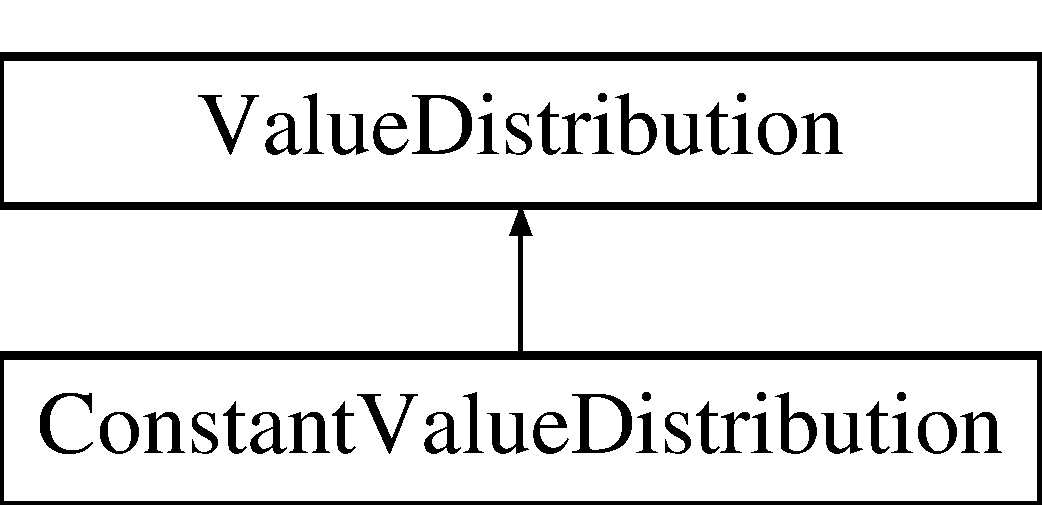
\includegraphics[height=2cm]{classConstantValueDistribution}
\end{center}
\end{figure}
\subsection*{Public Member Functions}
\begin{DoxyCompactItemize}
\item 
\hypertarget{classConstantValueDistribution_af232e63b78a2ecd39f1346d6d1db31c5}{
{\bfseries ConstantValueDistribution} (map$<$ string, string $>$ configuration)}
\label{classConstantValueDistribution_af232e63b78a2ecd39f1346d6d1db31c5}

\item 
\hypertarget{classConstantValueDistribution_a0e4c9a380df1cd2bde3d3267021b2071}{
string $\ast$ {\bfseries getNext} ()}
\label{classConstantValueDistribution_a0e4c9a380df1cd2bde3d3267021b2071}

\end{DoxyCompactItemize}


\subsection{Detailed Description}
Represents a value distribution with a fixed lenght 

The documentation for this class was generated from the following files:\begin{DoxyCompactItemize}
\item 
src/ConstantValueDistribution.h\item 
src/ConstantValueDistribution.cc\end{DoxyCompactItemize}

\hypertarget{classDummyKeyValueDB}{
\section{DummyKeyValueDB Class Reference}
\label{classDummyKeyValueDB}\index{DummyKeyValueDB@{DummyKeyValueDB}}
}


{\ttfamily \#include $<$DummyKeyValueDB.h$>$}Inheritance diagram for DummyKeyValueDB::\begin{figure}[H]
\begin{center}
\leavevmode
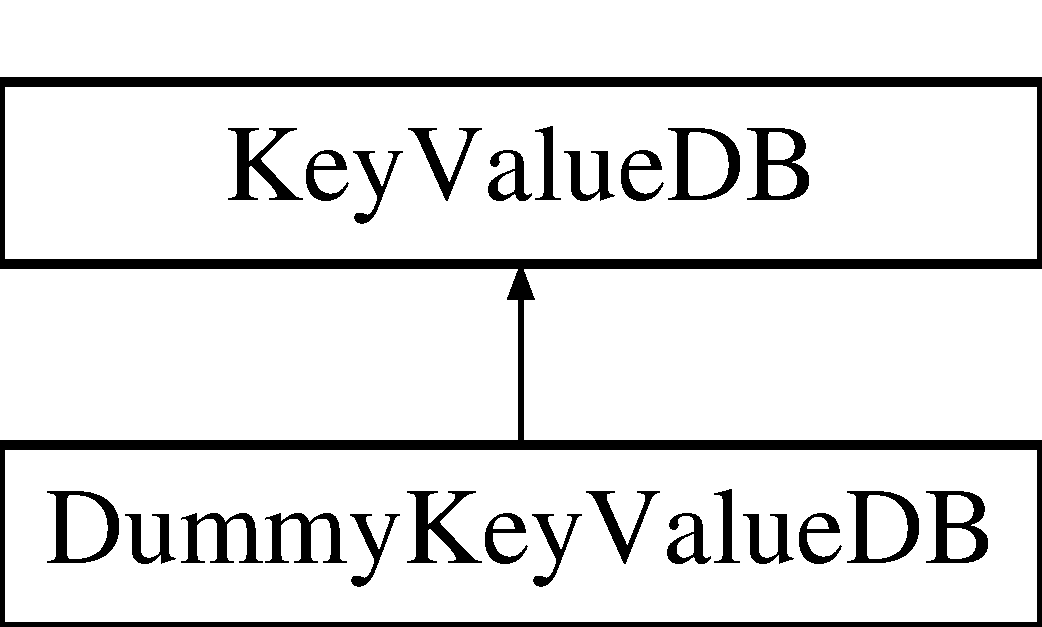
\includegraphics[height=2cm]{classDummyKeyValueDB}
\end{center}
\end{figure}


\subsection{Detailed Description}
Represents a key value database without any implementation in the backend This key value database is to be used when testing the performance of KeyValueClusterPerf itself 

The documentation for this class was generated from the following files:\begin{DoxyCompactItemize}
\item 
src/DummyKeyValueDB.h\item 
src/DummyKeyValueDB.cc\end{DoxyCompactItemize}

\hypertarget{classKeyValueDB}{
\section{KeyValueDB Class Reference}
\label{classKeyValueDB}\index{KeyValueDB@{KeyValueDB}}
}


{\ttfamily \#include $<$KeyValueDB.h$>$}Inheritance diagram for KeyValueDB::\begin{figure}[H]
\begin{center}
\leavevmode
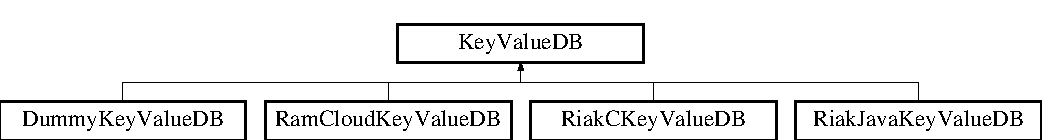
\includegraphics[height=1.87919cm]{classKeyValueDB}
\end{center}
\end{figure}
\subsection*{Public Member Functions}
\begin{DoxyCompactItemize}
\item 
\hypertarget{classKeyValueDB_a2b847092e0f3cac06b4e326661e9cd71}{
virtual void {\bfseries putValue} (string key, string $\ast$value)=0}
\label{classKeyValueDB_a2b847092e0f3cac06b4e326661e9cd71}

\item 
\hypertarget{classKeyValueDB_a651f01bff7dc8be6c68be6b3ec2ea519}{
virtual string {\bfseries getValue} (string key)=0}
\label{classKeyValueDB_a651f01bff7dc8be6c68be6b3ec2ea519}

\item 
\hypertarget{classKeyValueDB_a8431ec48c41b6c0cbfd2c2b8e8d13f4d}{
virtual void {\bfseries deleteValue} (string key)=0}
\label{classKeyValueDB_a8431ec48c41b6c0cbfd2c2b8e8d13f4d}

\item 
void \hyperlink{classKeyValueDB_aebd32f35aa2c11ac0d071bd8307fc521}{initialise} (map$<$ string, string $>$ keyValuePairs)
\end{DoxyCompactItemize}


\subsection{Detailed Description}
Abstract class representing all operations that a key value database should be able to perform Each key value database should use this class as a base 

\subsection{Member Function Documentation}
\hypertarget{classKeyValueDB_aebd32f35aa2c11ac0d071bd8307fc521}{
\index{KeyValueDB@{KeyValueDB}!initialise@{initialise}}
\index{initialise@{initialise}!KeyValueDB@{KeyValueDB}}
\subsubsection[{initialise}]{\setlength{\rightskip}{0pt plus 5cm}void KeyValueDB::initialise (map$<$ string, string $>$ {\em keyValuePairs})}}
\label{classKeyValueDB_aebd32f35aa2c11ac0d071bd8307fc521}
Initialise the key value database with the keyvalue-\/pairs represented by the map 

Reimplemented in \hyperlink{classRiakCKeyValueDB_ac57a6fe1e7b1d5759dcb43915d4f65da}{RiakCKeyValueDB}, and \hyperlink{classRiakJavaKeyValueDB_aa7e3df85b19f2c3a936a7282f8ddb98f}{RiakJavaKeyValueDB}.

The documentation for this class was generated from the following files:\begin{DoxyCompactItemize}
\item 
src/KeyValueDB.h\item 
src/KeyValueDB.cc\end{DoxyCompactItemize}

\hypertarget{classMessageSender}{
\section{MessageSender Class Reference}
\label{classMessageSender}\index{MessageSender@{MessageSender}}
}


{\ttfamily \#include $<$MessageSender.h$>$}\subsection*{Public Member Functions}
\begin{DoxyCompactItemize}
\item 
\hypertarget{classMessageSender_a9ed57cadd9393eca2b12f4cd51dbc8d2}{
void {\bfseries send} (string message)}
\label{classMessageSender_a9ed57cadd9393eca2b12f4cd51dbc8d2}

\item 
\hypertarget{classMessageSender_a89e7662e7e831865e8e9d1d602579418}{
string {\bfseries receive} ()}
\label{classMessageSender_a89e7662e7e831865e8e9d1d602579418}

\end{DoxyCompactItemize}


\subsection{Detailed Description}
Class responsible for all communication between the Java client of Riak and this C program 

The documentation for this class was generated from the following files:\begin{DoxyCompactItemize}
\item 
src/MessageSender.h\item 
src/MessageSender.cc\end{DoxyCompactItemize}

\hypertarget{classRamCloudKeyValueDB}{
\section{RamCloudKeyValueDB Class Reference}
\label{classRamCloudKeyValueDB}\index{RamCloudKeyValueDB@{RamCloudKeyValueDB}}
}


{\ttfamily \#include $<$RamCloudKeyValueDB.h$>$}Inheritance diagram for RamCloudKeyValueDB::\begin{figure}[H]
\begin{center}
\leavevmode
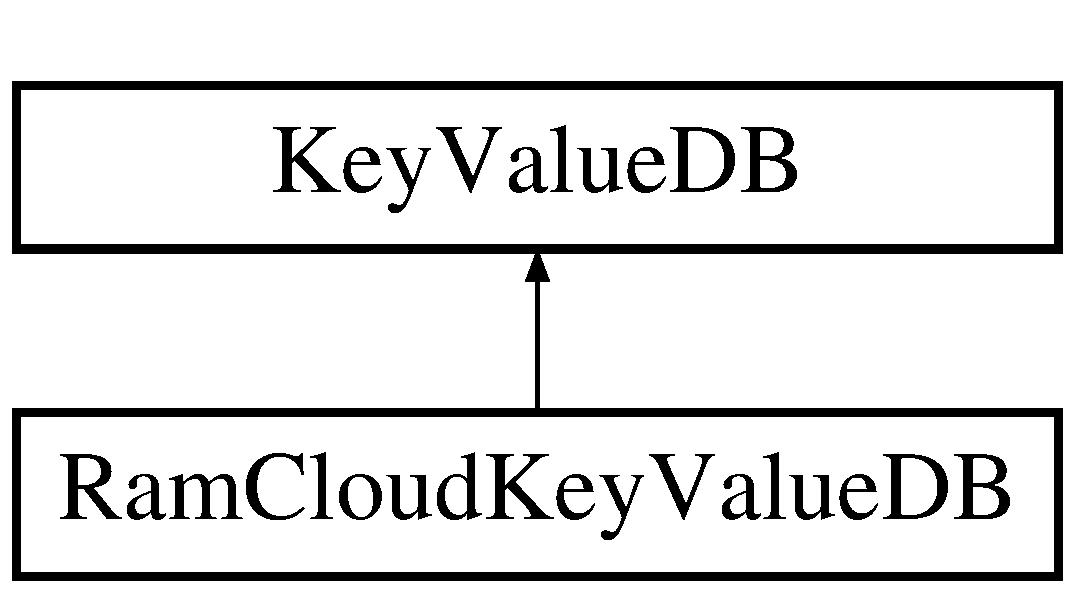
\includegraphics[height=2cm]{classRamCloudKeyValueDB}
\end{center}
\end{figure}
\subsection*{Public Member Functions}
\begin{DoxyCompactItemize}
\item 
\hypertarget{classRamCloudKeyValueDB_a597bb6fbbe622334c35cbe6a165bdb0f}{
{\bfseries RamCloudKeyValueDB} (map$<$ string, string $>$ configuration)}
\label{classRamCloudKeyValueDB_a597bb6fbbe622334c35cbe6a165bdb0f}

\item 
\hypertarget{classRamCloudKeyValueDB_a6e1b871add53feb0a0a738933df4898d}{
void {\bfseries putValue} (string key, string $\ast$value)}
\label{classRamCloudKeyValueDB_a6e1b871add53feb0a0a738933df4898d}

\item 
\hypertarget{classRamCloudKeyValueDB_ae46ce3504ba964b9d1f689111e67e495}{
string {\bfseries getValue} (string key)}
\label{classRamCloudKeyValueDB_ae46ce3504ba964b9d1f689111e67e495}

\item 
\hypertarget{classRamCloudKeyValueDB_abc2870c0eda566962c46b2ef6493addc}{
void {\bfseries deleteValue} (string key)}
\label{classRamCloudKeyValueDB_abc2870c0eda566962c46b2ef6493addc}

\end{DoxyCompactItemize}


\subsection{Detailed Description}
Class handling all key value database operations on a RamCloud cluster 

The documentation for this class was generated from the following files:\begin{DoxyCompactItemize}
\item 
src/RamCloudKeyValueDB.h\item 
src/RamCloudKeyValueDB.cc\end{DoxyCompactItemize}

\hypertarget{classRandomAccessPattern}{
\section{RandomAccessPattern Class Reference}
\label{classRandomAccessPattern}\index{RandomAccessPattern@{RandomAccessPattern}}
}


{\ttfamily \#include $<$RandomAccessPattern.h$>$}Inheritance diagram for RandomAccessPattern::\begin{figure}[H]
\begin{center}
\leavevmode
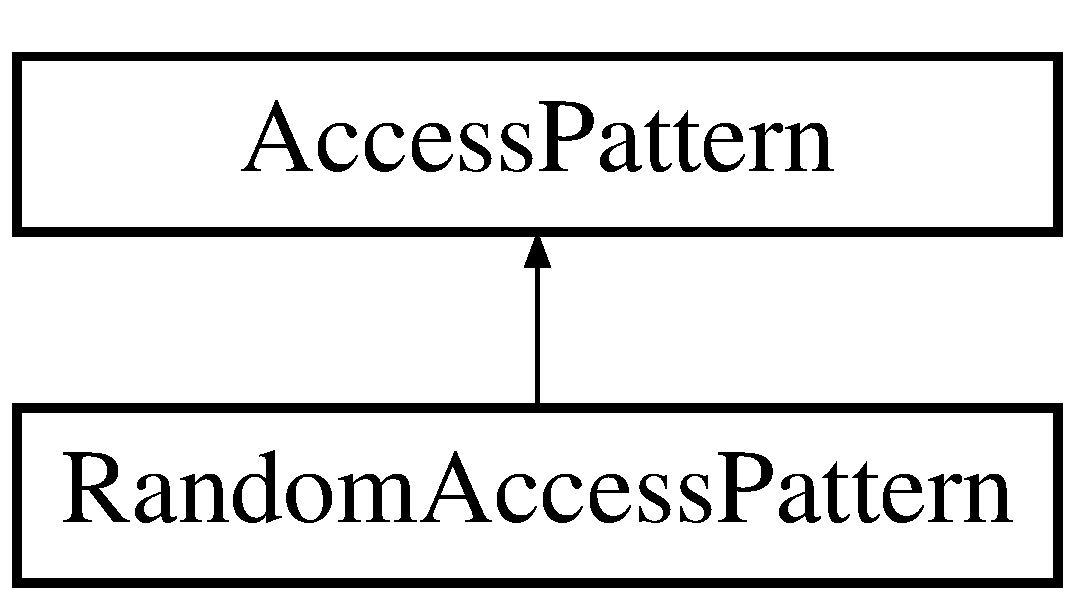
\includegraphics[height=2cm]{classRandomAccessPattern}
\end{center}
\end{figure}
\subsection*{Public Member Functions}
\begin{DoxyCompactItemize}
\item 
\hypertarget{classRandomAccessPattern_ad0dc7a4ff575c695277f449df68912c0}{
{\bfseries RandomAccessPattern} (map$<$ string, string $>$ configuration)}
\label{classRandomAccessPattern_ad0dc7a4ff575c695277f449df68912c0}

\item 
\hyperlink{structSingleAccess}{SingleAccess} \hyperlink{classRandomAccessPattern_a5b590afc37a8bf5e4a4235834c6ebe12}{getNext} ()
\item 
map$<$ string, string $>$ \hyperlink{classRandomAccessPattern_a72da825a9cb74f58fcadf6fc894d5e82}{getInitialisationKeyValuePairs} ()
\end{DoxyCompactItemize}


\subsection{Detailed Description}
Access pattern representing randomness in the keys and the read-\/write cycles 

\subsection{Member Function Documentation}
\hypertarget{classRandomAccessPattern_a72da825a9cb74f58fcadf6fc894d5e82}{
\index{RandomAccessPattern@{RandomAccessPattern}!getInitialisationKeyValuePairs@{getInitialisationKeyValuePairs}}
\index{getInitialisationKeyValuePairs@{getInitialisationKeyValuePairs}!RandomAccessPattern@{RandomAccessPattern}}
\subsubsection[{getInitialisationKeyValuePairs}]{\setlength{\rightskip}{0pt plus 5cm}map$<$ string, string $>$ RandomAccessPattern::getInitialisationKeyValuePairs ()\hspace{0.3cm}{\ttfamily  \mbox{[}virtual\mbox{]}}}}
\label{classRandomAccessPattern_a72da825a9cb74f58fcadf6fc894d5e82}
get key-\/value pairs to initialise database before simulation. This prevents access to non-\/existend items 

Implements \hyperlink{classAccessPattern_afa72bed11401bfd96e8fa88acd72934b}{AccessPattern}.\hypertarget{classRandomAccessPattern_a5b590afc37a8bf5e4a4235834c6ebe12}{
\index{RandomAccessPattern@{RandomAccessPattern}!getNext@{getNext}}
\index{getNext@{getNext}!RandomAccessPattern@{RandomAccessPattern}}
\subsubsection[{getNext}]{\setlength{\rightskip}{0pt plus 5cm}{\bf SingleAccess} RandomAccessPattern::getNext ()\hspace{0.3cm}{\ttfamily  \mbox{[}virtual\mbox{]}}}}
\label{classRandomAccessPattern_a5b590afc37a8bf5e4a4235834c6ebe12}
generate the next access information to the database 

Implements \hyperlink{classAccessPattern_a8c46aedb717e862598524f250f23086f}{AccessPattern}.

The documentation for this class was generated from the following files:\begin{DoxyCompactItemize}
\item 
src/RandomAccessPattern.h\item 
src/RandomAccessPattern.cc\end{DoxyCompactItemize}

\hypertarget{classReadOnlyAccessPattern}{
\section{ReadOnlyAccessPattern Class Reference}
\label{classReadOnlyAccessPattern}\index{ReadOnlyAccessPattern@{ReadOnlyAccessPattern}}
}


{\ttfamily \#include $<$ReadOnlyAccessPattern.h$>$}Inheritance diagram for ReadOnlyAccessPattern::\begin{figure}[H]
\begin{center}
\leavevmode
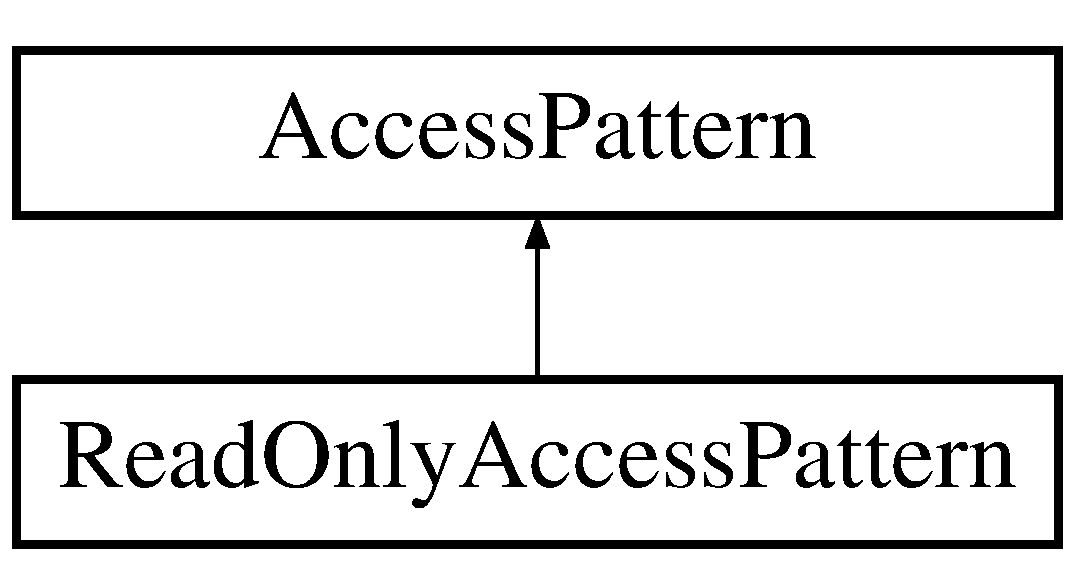
\includegraphics[height=2cm]{classReadOnlyAccessPattern}
\end{center}
\end{figure}
\subsection*{Public Member Functions}
\begin{DoxyCompactItemize}
\item 
\hypertarget{classReadOnlyAccessPattern_ac809863a35ba6cff81d7ae8e1b703bfa}{
{\bfseries ReadOnlyAccessPattern} (map$<$ string, string $>$ configuration)}
\label{classReadOnlyAccessPattern_ac809863a35ba6cff81d7ae8e1b703bfa}

\item 
\hyperlink{structSingleAccess}{SingleAccess} \hyperlink{classReadOnlyAccessPattern_a324b6da6296a17144d51db2841e16ba4}{getNext} ()
\item 
map$<$ string, string $>$ \hyperlink{classReadOnlyAccessPattern_a2e6ce8d90050b038ffbf643b344e0eb5}{getInitialisationKeyValuePairs} ()
\end{DoxyCompactItemize}


\subsection{Detailed Description}
Access pattern performing only reads 

\subsection{Member Function Documentation}
\hypertarget{classReadOnlyAccessPattern_a2e6ce8d90050b038ffbf643b344e0eb5}{
\index{ReadOnlyAccessPattern@{ReadOnlyAccessPattern}!getInitialisationKeyValuePairs@{getInitialisationKeyValuePairs}}
\index{getInitialisationKeyValuePairs@{getInitialisationKeyValuePairs}!ReadOnlyAccessPattern@{ReadOnlyAccessPattern}}
\subsubsection[{getInitialisationKeyValuePairs}]{\setlength{\rightskip}{0pt plus 5cm}map$<$ string, string $>$ ReadOnlyAccessPattern::getInitialisationKeyValuePairs ()\hspace{0.3cm}{\ttfamily  \mbox{[}virtual\mbox{]}}}}
\label{classReadOnlyAccessPattern_a2e6ce8d90050b038ffbf643b344e0eb5}
get key-\/value pairs to initialise database before simulation. This prevents access to non-\/existend items 

Implements \hyperlink{classAccessPattern_afa72bed11401bfd96e8fa88acd72934b}{AccessPattern}.\hypertarget{classReadOnlyAccessPattern_a324b6da6296a17144d51db2841e16ba4}{
\index{ReadOnlyAccessPattern@{ReadOnlyAccessPattern}!getNext@{getNext}}
\index{getNext@{getNext}!ReadOnlyAccessPattern@{ReadOnlyAccessPattern}}
\subsubsection[{getNext}]{\setlength{\rightskip}{0pt plus 5cm}{\bf SingleAccess} ReadOnlyAccessPattern::getNext ()\hspace{0.3cm}{\ttfamily  \mbox{[}virtual\mbox{]}}}}
\label{classReadOnlyAccessPattern_a324b6da6296a17144d51db2841e16ba4}
generate the next access information to the database 

Implements \hyperlink{classAccessPattern_a8c46aedb717e862598524f250f23086f}{AccessPattern}.

The documentation for this class was generated from the following files:\begin{DoxyCompactItemize}
\item 
src/ReadOnlyAccessPattern.h\item 
src/ReadOnlyAccessPattern.cc\end{DoxyCompactItemize}

\hypertarget{classmessaging_1_1RequestMessage}{
\section{messaging::RequestMessage Class Reference}
\label{classmessaging_1_1RequestMessage}\index{messaging::RequestMessage@{messaging::RequestMessage}}
}
\subsection*{Public Member Functions}
\begin{DoxyCompactItemize}
\item 
\hypertarget{classmessaging_1_1RequestMessage_a186291ebfb46715c9d915358a2ebb0e1}{
{\bfseries RequestMessage} (const \hyperlink{classmessaging_1_1RequestMessage}{RequestMessage} \&from)}
\label{classmessaging_1_1RequestMessage_a186291ebfb46715c9d915358a2ebb0e1}

\item 
\hypertarget{classmessaging_1_1RequestMessage_a23d7d6bcd46afd140ba1fad40d1bb62c}{
\hyperlink{classmessaging_1_1RequestMessage}{RequestMessage} \& {\bfseries operator=} (const \hyperlink{classmessaging_1_1RequestMessage}{RequestMessage} \&from)}
\label{classmessaging_1_1RequestMessage_a23d7d6bcd46afd140ba1fad40d1bb62c}

\item 
\hypertarget{classmessaging_1_1RequestMessage_a0919fbd2ccc35add6614ab7e60c0b9a5}{
const ::google::protobuf::UnknownFieldSet \& {\bfseries unknown\_\-fields} () const }
\label{classmessaging_1_1RequestMessage_a0919fbd2ccc35add6614ab7e60c0b9a5}

\item 
\hypertarget{classmessaging_1_1RequestMessage_a7a975a8941e7907f8801320e5f452f86}{
inline::google::protobuf::UnknownFieldSet $\ast$ {\bfseries mutable\_\-unknown\_\-fields} ()}
\label{classmessaging_1_1RequestMessage_a7a975a8941e7907f8801320e5f452f86}

\item 
\hypertarget{classmessaging_1_1RequestMessage_ab6249d7c52bdcb6509821dc40684dd63}{
void {\bfseries Swap} (\hyperlink{classmessaging_1_1RequestMessage}{RequestMessage} $\ast$other)}
\label{classmessaging_1_1RequestMessage_ab6249d7c52bdcb6509821dc40684dd63}

\item 
\hypertarget{classmessaging_1_1RequestMessage_a25255a09eb7941dd1fea92c9db3bc738}{
\hyperlink{classmessaging_1_1RequestMessage}{RequestMessage} $\ast$ {\bfseries New} () const }
\label{classmessaging_1_1RequestMessage_a25255a09eb7941dd1fea92c9db3bc738}

\item 
\hypertarget{classmessaging_1_1RequestMessage_af21b2d291d7b455505534c5607bd2ae4}{
void {\bfseries CopyFrom} (const ::google::protobuf::Message \&from)}
\label{classmessaging_1_1RequestMessage_af21b2d291d7b455505534c5607bd2ae4}

\item 
\hypertarget{classmessaging_1_1RequestMessage_ae400d288ac5dbc36cd48298e9fd3acb4}{
void {\bfseries MergeFrom} (const ::google::protobuf::Message \&from)}
\label{classmessaging_1_1RequestMessage_ae400d288ac5dbc36cd48298e9fd3acb4}

\item 
\hypertarget{classmessaging_1_1RequestMessage_a7e8370008cffba2a2322bc5cc074e4ce}{
void {\bfseries CopyFrom} (const \hyperlink{classmessaging_1_1RequestMessage}{RequestMessage} \&from)}
\label{classmessaging_1_1RequestMessage_a7e8370008cffba2a2322bc5cc074e4ce}

\item 
\hypertarget{classmessaging_1_1RequestMessage_ab8ef15832bfc6fb40b5d418f03a49b79}{
void {\bfseries MergeFrom} (const \hyperlink{classmessaging_1_1RequestMessage}{RequestMessage} \&from)}
\label{classmessaging_1_1RequestMessage_ab8ef15832bfc6fb40b5d418f03a49b79}

\item 
\hypertarget{classmessaging_1_1RequestMessage_af4e5735fe5e219f63096b2f1ab87d482}{
void {\bfseries Clear} ()}
\label{classmessaging_1_1RequestMessage_af4e5735fe5e219f63096b2f1ab87d482}

\item 
\hypertarget{classmessaging_1_1RequestMessage_a56ae2011121293a190a2b1ae0b038041}{
bool {\bfseries IsInitialized} () const }
\label{classmessaging_1_1RequestMessage_a56ae2011121293a190a2b1ae0b038041}

\item 
\hypertarget{classmessaging_1_1RequestMessage_ad9235b3f3595be9d49ec28fe652b84f6}{
int {\bfseries ByteSize} () const }
\label{classmessaging_1_1RequestMessage_ad9235b3f3595be9d49ec28fe652b84f6}

\item 
\hypertarget{classmessaging_1_1RequestMessage_abddbbad2b780085846220e4edfd2eab0}{
bool {\bfseries MergePartialFromCodedStream} (::google::protobuf::io::CodedInputStream $\ast$input)}
\label{classmessaging_1_1RequestMessage_abddbbad2b780085846220e4edfd2eab0}

\item 
\hypertarget{classmessaging_1_1RequestMessage_a19f22ff4b311eda48a372c01e5cce445}{
void {\bfseries SerializeWithCachedSizes} (::google::protobuf::io::CodedOutputStream $\ast$output) const }
\label{classmessaging_1_1RequestMessage_a19f22ff4b311eda48a372c01e5cce445}

\item 
\hypertarget{classmessaging_1_1RequestMessage_ae4f3186bcbc25dcf4c8b3241642dcdbb}{
::google::protobuf::uint8 $\ast$ {\bfseries SerializeWithCachedSizesToArray} (::google::protobuf::uint8 $\ast$output) const }
\label{classmessaging_1_1RequestMessage_ae4f3186bcbc25dcf4c8b3241642dcdbb}

\item 
\hypertarget{classmessaging_1_1RequestMessage_a1b156b4dc4f856376d1376861096c829}{
int {\bfseries GetCachedSize} () const }
\label{classmessaging_1_1RequestMessage_a1b156b4dc4f856376d1376861096c829}

\item 
\hypertarget{classmessaging_1_1RequestMessage_a00d6eeb34990997c363494e3b5d6fb26}{
::google::protobuf::Metadata {\bfseries GetMetadata} () const }
\label{classmessaging_1_1RequestMessage_a00d6eeb34990997c363494e3b5d6fb26}

\item 
\hypertarget{classmessaging_1_1RequestMessage_ad797d501aea6cc6db87b114ba1bd28b1}{
bool {\bfseries has\_\-command} () const }
\label{classmessaging_1_1RequestMessage_ad797d501aea6cc6db87b114ba1bd28b1}

\item 
\hypertarget{classmessaging_1_1RequestMessage_afa8ca59bd22a7fab3848224fe5bb2d7e}{
void {\bfseries clear\_\-command} ()}
\label{classmessaging_1_1RequestMessage_afa8ca59bd22a7fab3848224fe5bb2d7e}

\item 
\hypertarget{classmessaging_1_1RequestMessage_a1a4c684e33145f49257817e8e2d0c096}{
const ::std::string \& {\bfseries command} () const }
\label{classmessaging_1_1RequestMessage_a1a4c684e33145f49257817e8e2d0c096}

\item 
\hypertarget{classmessaging_1_1RequestMessage_a0a54cf196827d180f906c4ef4a6cebfa}{
void {\bfseries set\_\-command} (const ::std::string \&value)}
\label{classmessaging_1_1RequestMessage_a0a54cf196827d180f906c4ef4a6cebfa}

\item 
\hypertarget{classmessaging_1_1RequestMessage_a7e61a06625d579067dd561749ccd9d4d}{
void {\bfseries set\_\-command} (const char $\ast$value)}
\label{classmessaging_1_1RequestMessage_a7e61a06625d579067dd561749ccd9d4d}

\item 
\hypertarget{classmessaging_1_1RequestMessage_a485f242035c9b88218d75986e5d5cef6}{
void {\bfseries set\_\-command} (const char $\ast$value, size\_\-t size)}
\label{classmessaging_1_1RequestMessage_a485f242035c9b88218d75986e5d5cef6}

\item 
\hypertarget{classmessaging_1_1RequestMessage_a005e89188da50a30d74180ea5a7b41de}{
inline::std::string $\ast$ {\bfseries mutable\_\-command} ()}
\label{classmessaging_1_1RequestMessage_a005e89188da50a30d74180ea5a7b41de}

\item 
\hypertarget{classmessaging_1_1RequestMessage_a7aad456a9a8603097015e349202c43cd}{
inline::std::string $\ast$ {\bfseries release\_\-command} ()}
\label{classmessaging_1_1RequestMessage_a7aad456a9a8603097015e349202c43cd}

\item 
\hypertarget{classmessaging_1_1RequestMessage_a3376222000ea73aab5aa2820f75a4739}{
void {\bfseries set\_\-allocated\_\-command} (::std::string $\ast$command)}
\label{classmessaging_1_1RequestMessage_a3376222000ea73aab5aa2820f75a4739}

\item 
\hypertarget{classmessaging_1_1RequestMessage_a186ba1c789dab9f0dcdf7871a9cd5cd8}{
bool {\bfseries has\_\-key} () const }
\label{classmessaging_1_1RequestMessage_a186ba1c789dab9f0dcdf7871a9cd5cd8}

\item 
\hypertarget{classmessaging_1_1RequestMessage_a6fa549a415f20dcb92fc994007b246dc}{
void {\bfseries clear\_\-key} ()}
\label{classmessaging_1_1RequestMessage_a6fa549a415f20dcb92fc994007b246dc}

\item 
\hypertarget{classmessaging_1_1RequestMessage_af357f48e8e3ae4f2f34de028d50ebce6}{
const ::std::string \& {\bfseries key} () const }
\label{classmessaging_1_1RequestMessage_af357f48e8e3ae4f2f34de028d50ebce6}

\item 
\hypertarget{classmessaging_1_1RequestMessage_ab31cbe5ef09328c10198709b386bb09e}{
void {\bfseries set\_\-key} (const ::std::string \&value)}
\label{classmessaging_1_1RequestMessage_ab31cbe5ef09328c10198709b386bb09e}

\item 
\hypertarget{classmessaging_1_1RequestMessage_ad44fade1f8c326aa3660b307a3ad20f8}{
void {\bfseries set\_\-key} (const char $\ast$value)}
\label{classmessaging_1_1RequestMessage_ad44fade1f8c326aa3660b307a3ad20f8}

\item 
\hypertarget{classmessaging_1_1RequestMessage_a88b1064ca0989d92919f4ed9da5c1c8b}{
void {\bfseries set\_\-key} (const char $\ast$value, size\_\-t size)}
\label{classmessaging_1_1RequestMessage_a88b1064ca0989d92919f4ed9da5c1c8b}

\item 
\hypertarget{classmessaging_1_1RequestMessage_a6efcd1be041230b67d450c6fe4bc43ce}{
inline::std::string $\ast$ {\bfseries mutable\_\-key} ()}
\label{classmessaging_1_1RequestMessage_a6efcd1be041230b67d450c6fe4bc43ce}

\item 
\hypertarget{classmessaging_1_1RequestMessage_a43311ee7d4291e895ac0abd9b780f646}{
inline::std::string $\ast$ {\bfseries release\_\-key} ()}
\label{classmessaging_1_1RequestMessage_a43311ee7d4291e895ac0abd9b780f646}

\item 
\hypertarget{classmessaging_1_1RequestMessage_a49c65161742239387292d697f4052910}{
void {\bfseries set\_\-allocated\_\-key} (::std::string $\ast$key)}
\label{classmessaging_1_1RequestMessage_a49c65161742239387292d697f4052910}

\item 
\hypertarget{classmessaging_1_1RequestMessage_a6b6f689d2a22f3a17f091f5d70247728}{
bool {\bfseries has\_\-value} () const }
\label{classmessaging_1_1RequestMessage_a6b6f689d2a22f3a17f091f5d70247728}

\item 
\hypertarget{classmessaging_1_1RequestMessage_a11f2b8fe61fbb89bb18c73a44bc74283}{
void {\bfseries clear\_\-value} ()}
\label{classmessaging_1_1RequestMessage_a11f2b8fe61fbb89bb18c73a44bc74283}

\item 
\hypertarget{classmessaging_1_1RequestMessage_a3e310649fb8f672c4204ab6bfaab9bef}{
const ::std::string \& {\bfseries value} () const }
\label{classmessaging_1_1RequestMessage_a3e310649fb8f672c4204ab6bfaab9bef}

\item 
\hypertarget{classmessaging_1_1RequestMessage_a5a9a83ae66ea055ffc1fe6626fe834f9}{
void {\bfseries set\_\-value} (const ::std::string \&value)}
\label{classmessaging_1_1RequestMessage_a5a9a83ae66ea055ffc1fe6626fe834f9}

\item 
\hypertarget{classmessaging_1_1RequestMessage_aa30d4c7d9510ee9c4eb725136bf81433}{
void {\bfseries set\_\-value} (const char $\ast$value)}
\label{classmessaging_1_1RequestMessage_aa30d4c7d9510ee9c4eb725136bf81433}

\item 
\hypertarget{classmessaging_1_1RequestMessage_a65e297f82439202d87feee10a22ce578}{
void {\bfseries set\_\-value} (const char $\ast$value, size\_\-t size)}
\label{classmessaging_1_1RequestMessage_a65e297f82439202d87feee10a22ce578}

\item 
\hypertarget{classmessaging_1_1RequestMessage_a0bf14996bbccb2ccefece4ec01043b19}{
inline::std::string $\ast$ {\bfseries mutable\_\-value} ()}
\label{classmessaging_1_1RequestMessage_a0bf14996bbccb2ccefece4ec01043b19}

\item 
\hypertarget{classmessaging_1_1RequestMessage_ad332472c1ba8f27947d64c67acec43bc}{
inline::std::string $\ast$ {\bfseries release\_\-value} ()}
\label{classmessaging_1_1RequestMessage_ad332472c1ba8f27947d64c67acec43bc}

\item 
\hypertarget{classmessaging_1_1RequestMessage_a052f73b263cd7ab615fba21517868904}{
void {\bfseries set\_\-allocated\_\-value} (::std::string $\ast$value)}
\label{classmessaging_1_1RequestMessage_a052f73b263cd7ab615fba21517868904}

\item 
\hypertarget{classmessaging_1_1RequestMessage_a3d271a6e08e4c9a1003171a4bde73ceb}{
bool {\bfseries has\_\-error} () const }
\label{classmessaging_1_1RequestMessage_a3d271a6e08e4c9a1003171a4bde73ceb}

\item 
\hypertarget{classmessaging_1_1RequestMessage_a5de4b70d34bc22abf6bb2908dc29f524}{
void {\bfseries clear\_\-error} ()}
\label{classmessaging_1_1RequestMessage_a5de4b70d34bc22abf6bb2908dc29f524}

\item 
\hypertarget{classmessaging_1_1RequestMessage_a0aa8c57effb530e12edbd126d0b611d9}{
const ::std::string \& {\bfseries error} () const }
\label{classmessaging_1_1RequestMessage_a0aa8c57effb530e12edbd126d0b611d9}

\item 
\hypertarget{classmessaging_1_1RequestMessage_a28cec88a92df69e45ec7c3ef5e0b4478}{
void {\bfseries set\_\-error} (const ::std::string \&value)}
\label{classmessaging_1_1RequestMessage_a28cec88a92df69e45ec7c3ef5e0b4478}

\item 
\hypertarget{classmessaging_1_1RequestMessage_ac21e265e31d85c023ff66766e7acea75}{
void {\bfseries set\_\-error} (const char $\ast$value)}
\label{classmessaging_1_1RequestMessage_ac21e265e31d85c023ff66766e7acea75}

\item 
\hypertarget{classmessaging_1_1RequestMessage_a3c8475cddab9bda40260e1481061867b}{
void {\bfseries set\_\-error} (const char $\ast$value, size\_\-t size)}
\label{classmessaging_1_1RequestMessage_a3c8475cddab9bda40260e1481061867b}

\item 
\hypertarget{classmessaging_1_1RequestMessage_a6c0021c35cf315cdd62c58b9cc1a0492}{
inline::std::string $\ast$ {\bfseries mutable\_\-error} ()}
\label{classmessaging_1_1RequestMessage_a6c0021c35cf315cdd62c58b9cc1a0492}

\item 
\hypertarget{classmessaging_1_1RequestMessage_a82d180964442f2bcfd3357d690f9437b}{
inline::std::string $\ast$ {\bfseries release\_\-error} ()}
\label{classmessaging_1_1RequestMessage_a82d180964442f2bcfd3357d690f9437b}

\item 
\hypertarget{classmessaging_1_1RequestMessage_a7a0c0f9be6df1d35fa465815bc9d864c}{
void {\bfseries set\_\-allocated\_\-error} (::std::string $\ast$error)}
\label{classmessaging_1_1RequestMessage_a7a0c0f9be6df1d35fa465815bc9d864c}

\end{DoxyCompactItemize}
\subsection*{Static Public Member Functions}
\begin{DoxyCompactItemize}
\item 
\hypertarget{classmessaging_1_1RequestMessage_afddf1eabd783d362023788567f7c7531}{
static const ::google::protobuf::Descriptor $\ast$ {\bfseries descriptor} ()}
\label{classmessaging_1_1RequestMessage_afddf1eabd783d362023788567f7c7531}

\item 
\hypertarget{classmessaging_1_1RequestMessage_aea492c54cdb9f8f5c22ebb1b01cc467b}{
static const \hyperlink{classmessaging_1_1RequestMessage}{RequestMessage} \& {\bfseries default\_\-instance} ()}
\label{classmessaging_1_1RequestMessage_aea492c54cdb9f8f5c22ebb1b01cc467b}

\end{DoxyCompactItemize}
\subsection*{Static Public Attributes}
\begin{DoxyCompactItemize}
\item 
\hypertarget{classmessaging_1_1RequestMessage_a0c270411775903d07b58c6a5f865a3f8}{
static const int {\bfseries kCommandFieldNumber} = 1}
\label{classmessaging_1_1RequestMessage_a0c270411775903d07b58c6a5f865a3f8}

\item 
\hypertarget{classmessaging_1_1RequestMessage_a45d521e094860d2d622b17b5975282a5}{
static const int {\bfseries kKeyFieldNumber} = 2}
\label{classmessaging_1_1RequestMessage_a45d521e094860d2d622b17b5975282a5}

\item 
\hypertarget{classmessaging_1_1RequestMessage_a4fbfbd44dc0ea50f4a8f197895ad93ba}{
static const int {\bfseries kValueFieldNumber} = 3}
\label{classmessaging_1_1RequestMessage_a4fbfbd44dc0ea50f4a8f197895ad93ba}

\item 
\hypertarget{classmessaging_1_1RequestMessage_a4557cc932a5964f9827b3c2c9c52ab66}{
static const int {\bfseries kErrorFieldNumber} = 4}
\label{classmessaging_1_1RequestMessage_a4557cc932a5964f9827b3c2c9c52ab66}

\end{DoxyCompactItemize}
\subsection*{Friends}
\begin{DoxyCompactItemize}
\item 
\hypertarget{classmessaging_1_1RequestMessage_a02a86ef57244d57785784c27ff592220}{
void {\bfseries protobuf\_\-AddDesc\_\-request\_\-2eproto} ()}
\label{classmessaging_1_1RequestMessage_a02a86ef57244d57785784c27ff592220}

\item 
\hypertarget{classmessaging_1_1RequestMessage_a7d9c7404130d39c1e3e4e21fb2ffefb4}{
void {\bfseries protobuf\_\-AssignDesc\_\-request\_\-2eproto} ()}
\label{classmessaging_1_1RequestMessage_a7d9c7404130d39c1e3e4e21fb2ffefb4}

\item 
\hypertarget{classmessaging_1_1RequestMessage_a11a96ccaf635e1f5d5668b1055933760}{
void {\bfseries protobuf\_\-ShutdownFile\_\-request\_\-2eproto} ()}
\label{classmessaging_1_1RequestMessage_a11a96ccaf635e1f5d5668b1055933760}

\end{DoxyCompactItemize}


The documentation for this class was generated from the following files:\begin{DoxyCompactItemize}
\item 
src/request.pb.h\item 
src/request.pb.cc\end{DoxyCompactItemize}

\hypertarget{classRiakCKeyValueDB}{
\section{RiakCKeyValueDB Class Reference}
\label{classRiakCKeyValueDB}\index{RiakCKeyValueDB@{RiakCKeyValueDB}}
}


{\ttfamily \#include $<$RiakCKeyValueDB.h$>$}Inheritance diagram for RiakCKeyValueDB::\begin{figure}[H]
\begin{center}
\leavevmode
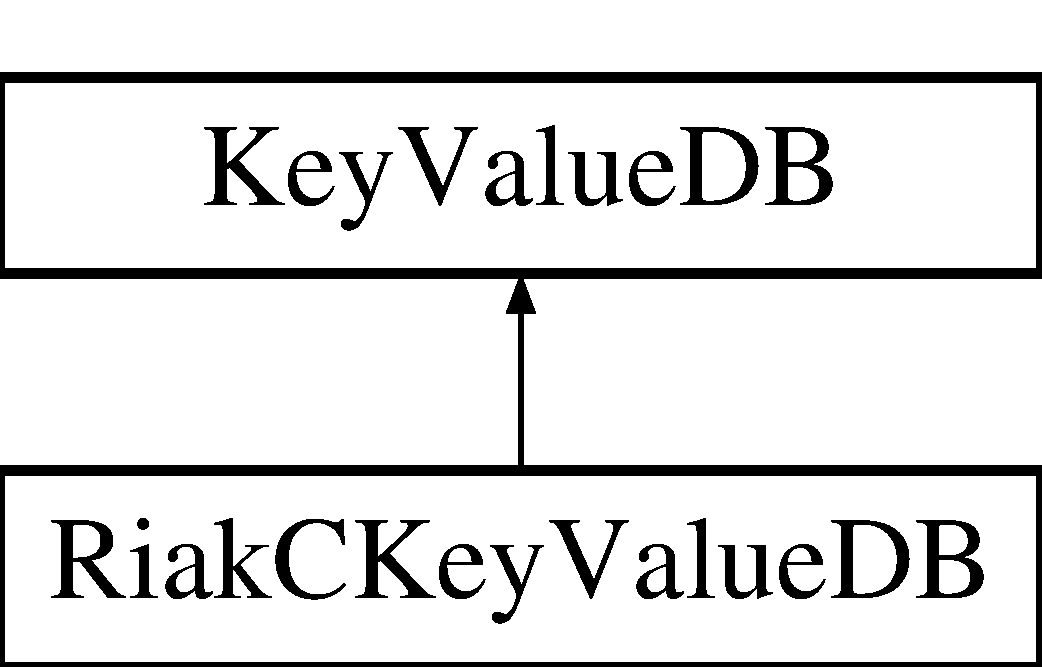
\includegraphics[height=2cm]{classRiakCKeyValueDB}
\end{center}
\end{figure}
\subsection*{Public Member Functions}
\begin{DoxyCompactItemize}
\item 
\hypertarget{classRiakCKeyValueDB_ad035ea0943d0ce5d1ee2fae2a13f6b78}{
{\bfseries RiakCKeyValueDB} (map$<$ string, string $>$ configuration)}
\label{classRiakCKeyValueDB_ad035ea0943d0ce5d1ee2fae2a13f6b78}

\item 
\hypertarget{classRiakCKeyValueDB_a651f7b83c0ae06751515661cc863ca6b}{
void {\bfseries putValue} (string key, string $\ast$value)}
\label{classRiakCKeyValueDB_a651f7b83c0ae06751515661cc863ca6b}

\item 
\hypertarget{classRiakCKeyValueDB_aa94128187a465b6526192e1d06fb084c}{
string {\bfseries getValue} (string key)}
\label{classRiakCKeyValueDB_aa94128187a465b6526192e1d06fb084c}

\item 
\hypertarget{classRiakCKeyValueDB_a513f70656d6b625bb48bf24721a3cac9}{
void {\bfseries deleteValue} (string key)}
\label{classRiakCKeyValueDB_a513f70656d6b625bb48bf24721a3cac9}

\item 
void \hyperlink{classRiakCKeyValueDB_ac57a6fe1e7b1d5759dcb43915d4f65da}{initialise} (map$<$ string, string $>$ keyValuePairs)
\end{DoxyCompactItemize}


\subsection{Detailed Description}
Class containing all functionality to communicate with a Riak cluster using C 

\subsection{Member Function Documentation}
\hypertarget{classRiakCKeyValueDB_ac57a6fe1e7b1d5759dcb43915d4f65da}{
\index{RiakCKeyValueDB@{RiakCKeyValueDB}!initialise@{initialise}}
\index{initialise@{initialise}!RiakCKeyValueDB@{RiakCKeyValueDB}}
\subsubsection[{initialise}]{\setlength{\rightskip}{0pt plus 5cm}void RiakCKeyValueDB::initialise (map$<$ string, string $>$ {\em keyValuePairs})}}
\label{classRiakCKeyValueDB_ac57a6fe1e7b1d5759dcb43915d4f65da}
Initialise the key value database with the keyvalue-\/pairs represented by the map 

Reimplemented from \hyperlink{classKeyValueDB_aebd32f35aa2c11ac0d071bd8307fc521}{KeyValueDB}.

The documentation for this class was generated from the following files:\begin{DoxyCompactItemize}
\item 
src/RiakCKeyValueDB.h\item 
src/RiakCKeyValueDB.cc\end{DoxyCompactItemize}

\hypertarget{classRiakJavaKeyValueDB}{
\section{RiakJavaKeyValueDB Class Reference}
\label{classRiakJavaKeyValueDB}\index{RiakJavaKeyValueDB@{RiakJavaKeyValueDB}}
}


{\ttfamily \#include $<$RiakJavaKeyValueDB.h$>$}Inheritance diagram for RiakJavaKeyValueDB::\begin{figure}[H]
\begin{center}
\leavevmode
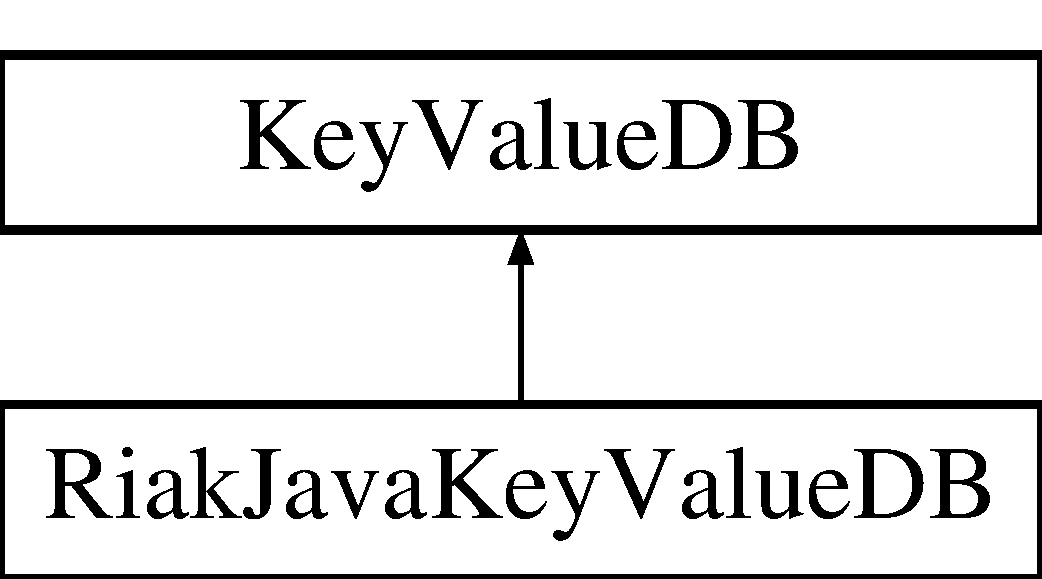
\includegraphics[height=2cm]{classRiakJavaKeyValueDB}
\end{center}
\end{figure}
\subsection*{Public Member Functions}
\begin{DoxyCompactItemize}
\item 
\hypertarget{classRiakJavaKeyValueDB_ac2b73488926b960d8d76eac2575ff886}{
{\bfseries RiakJavaKeyValueDB} (map$<$ string, string $>$ configuration)}
\label{classRiakJavaKeyValueDB_ac2b73488926b960d8d76eac2575ff886}

\item 
\hypertarget{classRiakJavaKeyValueDB_ad9bb63fe88d2d7baf89adb3e13afc8c3}{
void {\bfseries putValue} (string key, string $\ast$value)}
\label{classRiakJavaKeyValueDB_ad9bb63fe88d2d7baf89adb3e13afc8c3}

\item 
\hypertarget{classRiakJavaKeyValueDB_a5ed0606feebc3fa7f4997b3048dbb4f9}{
string {\bfseries getValue} (string key)}
\label{classRiakJavaKeyValueDB_a5ed0606feebc3fa7f4997b3048dbb4f9}

\item 
\hypertarget{classRiakJavaKeyValueDB_af228bd73a99e8c7ea138a8dad2a0e4cd}{
void {\bfseries deleteValue} (string key)}
\label{classRiakJavaKeyValueDB_af228bd73a99e8c7ea138a8dad2a0e4cd}

\item 
void \hyperlink{classRiakJavaKeyValueDB_aa7e3df85b19f2c3a936a7282f8ddb98f}{initialise} (map$<$ string, string $>$ keyValuePairs)
\end{DoxyCompactItemize}


\subsection{Detailed Description}
Class containing functionality to perform key value operations on a Riak cluster using a Java client 

\subsection{Member Function Documentation}
\hypertarget{classRiakJavaKeyValueDB_aa7e3df85b19f2c3a936a7282f8ddb98f}{
\index{RiakJavaKeyValueDB@{RiakJavaKeyValueDB}!initialise@{initialise}}
\index{initialise@{initialise}!RiakJavaKeyValueDB@{RiakJavaKeyValueDB}}
\subsubsection[{initialise}]{\setlength{\rightskip}{0pt plus 5cm}void RiakJavaKeyValueDB::initialise (map$<$ string, string $>$ {\em keyValuePairs})}}
\label{classRiakJavaKeyValueDB_aa7e3df85b19f2c3a936a7282f8ddb98f}
Initialise the key value database with the keyvalue-\/pairs represented by the map 

Reimplemented from \hyperlink{classKeyValueDB_aebd32f35aa2c11ac0d071bd8307fc521}{KeyValueDB}.

The documentation for this class was generated from the following files:\begin{DoxyCompactItemize}
\item 
src/RiakJavaKeyValueDB.h\item 
src/RiakJavaKeyValueDB.cc\end{DoxyCompactItemize}

\hypertarget{classSimulationController}{
\section{SimulationController Class Reference}
\label{classSimulationController}\index{SimulationController@{SimulationController}}
}


{\ttfamily \#include $<$SimulationController.h$>$}\subsection*{Public Member Functions}
\begin{DoxyCompactItemize}
\item 
\hypertarget{classSimulationController_ad3842750a34161c40e2503601d0d7261}{
{\bfseries SimulationController} (string hostFilePath, int hostLimit, int simIteration)}
\label{classSimulationController_ad3842750a34161c40e2503601d0d7261}

\item 
void \hyperlink{classSimulationController_a37b7e33fd9ea6d3505cc8ae1dbbbf284}{connect} ()
\item 
void \hyperlink{classSimulationController_a269e17c70a9661843bbd536d62dc771f}{disconnect} ()
\item 
void \hyperlink{classSimulationController_a5b756fb934ac05829b28e46a85a6497d}{execute} ()
\end{DoxyCompactItemize}


\subsection{Detailed Description}
Class handling the control of the entire simulation, instructing the worker nodes on the next task and merging the results. 

\subsection{Member Function Documentation}
\hypertarget{classSimulationController_a37b7e33fd9ea6d3505cc8ae1dbbbf284}{
\index{SimulationController@{SimulationController}!connect@{connect}}
\index{connect@{connect}!SimulationController@{SimulationController}}
\subsubsection[{connect}]{\setlength{\rightskip}{0pt plus 5cm}void SimulationController::connect ()}}
\label{classSimulationController_a37b7e33fd9ea6d3505cc8ae1dbbbf284}
Connect to all hosts specified in the host file \hypertarget{classSimulationController_a269e17c70a9661843bbd536d62dc771f}{
\index{SimulationController@{SimulationController}!disconnect@{disconnect}}
\index{disconnect@{disconnect}!SimulationController@{SimulationController}}
\subsubsection[{disconnect}]{\setlength{\rightskip}{0pt plus 5cm}void SimulationController::disconnect ()}}
\label{classSimulationController_a269e17c70a9661843bbd536d62dc771f}
Disconnect from the hosts \hypertarget{classSimulationController_a5b756fb934ac05829b28e46a85a6497d}{
\index{SimulationController@{SimulationController}!execute@{execute}}
\index{execute@{execute}!SimulationController@{SimulationController}}
\subsubsection[{execute}]{\setlength{\rightskip}{0pt plus 5cm}void SimulationController::execute ()}}
\label{classSimulationController_a5b756fb934ac05829b28e46a85a6497d}
Start the simulation by instructing the worker nodes 

The documentation for this class was generated from the following files:\begin{DoxyCompactItemize}
\item 
src/SimulationController.h\item 
src/SimulationController.cc\end{DoxyCompactItemize}

\hypertarget{classSimulationWorker}{
\section{SimulationWorker Class Reference}
\label{classSimulationWorker}\index{SimulationWorker@{SimulationWorker}}
}


{\ttfamily \#include $<$SimulationWorker.h$>$}\subsection*{Public Member Functions}
\begin{DoxyCompactItemize}
\item 
\hypertarget{classSimulationWorker_a44b25296237849bb3b8affad2956e87d}{
{\bfseries SimulationWorker} (string databaseCfgPath, string accessPatternCfgPath, string valueDistributionCfgPath, bool skipInit)}
\label{classSimulationWorker_a44b25296237849bb3b8affad2956e87d}

\item 
void \hyperlink{classSimulationWorker_ac8e581d784c84d98db09c3261395d2ed}{openConnection} (int portNum, int dataportNum)
\item 
void \hyperlink{classSimulationWorker_aaccde1ec2e77fb934b67718c104e69e8}{closeConnection} ()
\item 
void \hyperlink{classSimulationWorker_a18064a1d65824d3c6a522cf68e52e3f5}{listen} ()
\item 
void \hyperlink{classSimulationWorker_aba581c4c9cbdaf10624822e687efd08e}{initialiseSimulator} ()
\item 
void \hyperlink{classSimulationWorker_aa415eb89cba4b39457faed0baa65458c}{deinitialiseSimulator} ()
\end{DoxyCompactItemize}


\subsection{Detailed Description}
Worker node performing the tasks according to a fixed pattern determined by the controller node 

\subsection{Member Function Documentation}
\hypertarget{classSimulationWorker_aaccde1ec2e77fb934b67718c104e69e8}{
\index{SimulationWorker@{SimulationWorker}!closeConnection@{closeConnection}}
\index{closeConnection@{closeConnection}!SimulationWorker@{SimulationWorker}}
\subsubsection[{closeConnection}]{\setlength{\rightskip}{0pt plus 5cm}void SimulationWorker::closeConnection ()}}
\label{classSimulationWorker_aaccde1ec2e77fb934b67718c104e69e8}
Close the connection to the controller \hypertarget{classSimulationWorker_aa415eb89cba4b39457faed0baa65458c}{
\index{SimulationWorker@{SimulationWorker}!deinitialiseSimulator@{deinitialiseSimulator}}
\index{deinitialiseSimulator@{deinitialiseSimulator}!SimulationWorker@{SimulationWorker}}
\subsubsection[{deinitialiseSimulator}]{\setlength{\rightskip}{0pt plus 5cm}void SimulationWorker::deinitialiseSimulator ()}}
\label{classSimulationWorker_aa415eb89cba4b39457faed0baa65458c}
Delete simulation object, only call when all hosts finished \hypertarget{classSimulationWorker_aba581c4c9cbdaf10624822e687efd08e}{
\index{SimulationWorker@{SimulationWorker}!initialiseSimulator@{initialiseSimulator}}
\index{initialiseSimulator@{initialiseSimulator}!SimulationWorker@{SimulationWorker}}
\subsubsection[{initialiseSimulator}]{\setlength{\rightskip}{0pt plus 5cm}void SimulationWorker::initialiseSimulator ()}}
\label{classSimulationWorker_aba581c4c9cbdaf10624822e687efd08e}
Create a simulationobject \hypertarget{classSimulationWorker_a18064a1d65824d3c6a522cf68e52e3f5}{
\index{SimulationWorker@{SimulationWorker}!listen@{listen}}
\index{listen@{listen}!SimulationWorker@{SimulationWorker}}
\subsubsection[{listen}]{\setlength{\rightskip}{0pt plus 5cm}void SimulationWorker::listen ()}}
\label{classSimulationWorker_a18064a1d65824d3c6a522cf68e52e3f5}
Listen for commands from the controller \hypertarget{classSimulationWorker_ac8e581d784c84d98db09c3261395d2ed}{
\index{SimulationWorker@{SimulationWorker}!openConnection@{openConnection}}
\index{openConnection@{openConnection}!SimulationWorker@{SimulationWorker}}
\subsubsection[{openConnection}]{\setlength{\rightskip}{0pt plus 5cm}void SimulationWorker::openConnection (int {\em portNum}, \/  int {\em dataportNum})}}
\label{classSimulationWorker_ac8e581d784c84d98db09c3261395d2ed}
Opens a port so that the controller can connect to it 

The documentation for this class was generated from the following files:\begin{DoxyCompactItemize}
\item 
src/SimulationWorker.h\item 
src/SimulationWorker.cc\end{DoxyCompactItemize}

\hypertarget{classSimulator}{
\section{Simulator Class Reference}
\label{classSimulator}\index{Simulator@{Simulator}}
}


{\ttfamily \#include $<$Simulator.h$>$}\subsection*{Public Member Functions}
\begin{DoxyCompactItemize}
\item 
\hyperlink{classSimulator_a5c46ca7ea1fd4a67fc43d931fadbb347}{Simulator} (map$<$ string, string $>$ databaseConfiguration, map$<$ string, string $>$ accessPatternConfiguration, map$<$ string, string $>$ valueDistributionConfiguration, bool skipInitialisation)
\item 
\hyperlink{classSimulator_a031573bfcfe2e0f5c9539bcc1c7fc5d9}{Simulator} ()
\item 
void \hyperlink{classSimulator_a833eb17dd0d0d1b0b1f7c0747032c21c}{simulate} (int runs)
\item 
void \hyperlink{classSimulator_a224de0acb821d6b4e333c1821bea57d9}{burnInOut} (int runs)
\item 
map$<$ string, string $>$ \hyperlink{classSimulator_a510b4c3d8d032e7b5abf12e2572a8c5b}{getResults} ()
\item 
void \hyperlink{classSimulator_a3c9f45bd002ee6b88b6ec4d55d65e0ff}{mergeResults} (list$<$ map$<$ string, string $>$$>$ results, string csvFilePath)
\end{DoxyCompactItemize}


\subsection{Detailed Description}
Class to perform the actual simulation and merge the results. Workers use this class to simulate, controllers to merge 

\subsection{Constructor \& Destructor Documentation}
\hypertarget{classSimulator_a5c46ca7ea1fd4a67fc43d931fadbb347}{
\index{Simulator@{Simulator}!Simulator@{Simulator}}
\index{Simulator@{Simulator}!Simulator@{Simulator}}
\subsubsection[{Simulator}]{\setlength{\rightskip}{0pt plus 5cm}Simulator::Simulator (map$<$ string, string $>$ {\em databaseConfiguration}, \/  map$<$ string, string $>$ {\em accessPatternConfiguration}, \/  map$<$ string, string $>$ {\em valueDistributionConfiguration}, \/  bool {\em skipInitialisation})}}
\label{classSimulator_a5c46ca7ea1fd4a67fc43d931fadbb347}
Constructor for worker node to pass the configuration \hypertarget{classSimulator_a031573bfcfe2e0f5c9539bcc1c7fc5d9}{
\index{Simulator@{Simulator}!Simulator@{Simulator}}
\index{Simulator@{Simulator}!Simulator@{Simulator}}
\subsubsection[{Simulator}]{\setlength{\rightskip}{0pt plus 5cm}Simulator::Simulator ()}}
\label{classSimulator_a031573bfcfe2e0f5c9539bcc1c7fc5d9}
Separate contructor for controller because it does not use any configuration 

\subsection{Member Function Documentation}
\hypertarget{classSimulator_a224de0acb821d6b4e333c1821bea57d9}{
\index{Simulator@{Simulator}!burnInOut@{burnInOut}}
\index{burnInOut@{burnInOut}!Simulator@{Simulator}}
\subsubsection[{burnInOut}]{\setlength{\rightskip}{0pt plus 5cm}void Simulator::burnInOut (int {\em runs})}}
\label{classSimulator_a224de0acb821d6b4e333c1821bea57d9}
Perform burn in or burn out, dous not count towards statistics \hypertarget{classSimulator_a510b4c3d8d032e7b5abf12e2572a8c5b}{
\index{Simulator@{Simulator}!getResults@{getResults}}
\index{getResults@{getResults}!Simulator@{Simulator}}
\subsubsection[{getResults}]{\setlength{\rightskip}{0pt plus 5cm}map$<$ string, string $>$ Simulator::getResults ()}}
\label{classSimulator_a510b4c3d8d032e7b5abf12e2572a8c5b}
Get the statistics results from the last simulation \hypertarget{classSimulator_a3c9f45bd002ee6b88b6ec4d55d65e0ff}{
\index{Simulator@{Simulator}!mergeResults@{mergeResults}}
\index{mergeResults@{mergeResults}!Simulator@{Simulator}}
\subsubsection[{mergeResults}]{\setlength{\rightskip}{0pt plus 5cm}void Simulator::mergeResults (list$<$ map$<$ string, string $>$$>$ {\em results}, \/  string {\em csvFilePath})}}
\label{classSimulator_a3c9f45bd002ee6b88b6ec4d55d65e0ff}
Merge the results of multiple simulators \hypertarget{classSimulator_a833eb17dd0d0d1b0b1f7c0747032c21c}{
\index{Simulator@{Simulator}!simulate@{simulate}}
\index{simulate@{simulate}!Simulator@{Simulator}}
\subsubsection[{simulate}]{\setlength{\rightskip}{0pt plus 5cm}void Simulator::simulate (int {\em runs})}}
\label{classSimulator_a833eb17dd0d0d1b0b1f7c0747032c21c}
start the simulation 

The documentation for this class was generated from the following files:\begin{DoxyCompactItemize}
\item 
src/Simulator.h\item 
src/Simulator.cc\end{DoxyCompactItemize}

\hypertarget{structSingleAccess}{
\section{SingleAccess Struct Reference}
\label{structSingleAccess}\index{SingleAccess@{SingleAccess}}
}


{\ttfamily \#include $<$AccessPattern.h$>$}\subsection*{Data Fields}
\begin{DoxyCompactItemize}
\item 
\hypertarget{structSingleAccess_a2e929c9bcb7bc195230f3ceea90028da}{
bool {\bfseries read}}
\label{structSingleAccess_a2e929c9bcb7bc195230f3ceea90028da}

\item 
\hypertarget{structSingleAccess_a96ac3bf0a548e0fe74d11ca3c7fd337d}{
string {\bfseries key}}
\label{structSingleAccess_a96ac3bf0a548e0fe74d11ca3c7fd337d}

\item 
\hypertarget{structSingleAccess_a427f0fee8c2bef6c7830811d95b86202}{
string $\ast$ {\bfseries value}}
\label{structSingleAccess_a427f0fee8c2bef6c7830811d95b86202}

\end{DoxyCompactItemize}


\subsection{Detailed Description}
A single access to the database is defined as a struct to increase speed and prevent memory errors It shows if it is a read or write operation, what the key is and a pointer to the value This value should not be cleared as it is owned and reused by the valueDistribution 

The documentation for this struct was generated from the following file:\begin{DoxyCompactItemize}
\item 
src/AccessPattern.h\end{DoxyCompactItemize}

\hypertarget{structmessaging_1_1StaticDescriptorInitializer__request__2eproto}{
\section{messaging::StaticDescriptorInitializer\_\-request\_\-2eproto Struct Reference}
\label{structmessaging_1_1StaticDescriptorInitializer__request__2eproto}\index{messaging::StaticDescriptorInitializer\_\-request\_\-2eproto@{messaging::StaticDescriptorInitializer\_\-request\_\-2eproto}}
}


The documentation for this struct was generated from the following file:\begin{DoxyCompactItemize}
\item 
src/request.pb.cc\end{DoxyCompactItemize}

\hypertarget{classValueDistribution}{
\section{ValueDistribution Class Reference}
\label{classValueDistribution}\index{ValueDistribution@{ValueDistribution}}
}


{\ttfamily \#include $<$ValueDistribution.h$>$}Inheritance diagram for ValueDistribution::\begin{figure}[H]
\begin{center}
\leavevmode
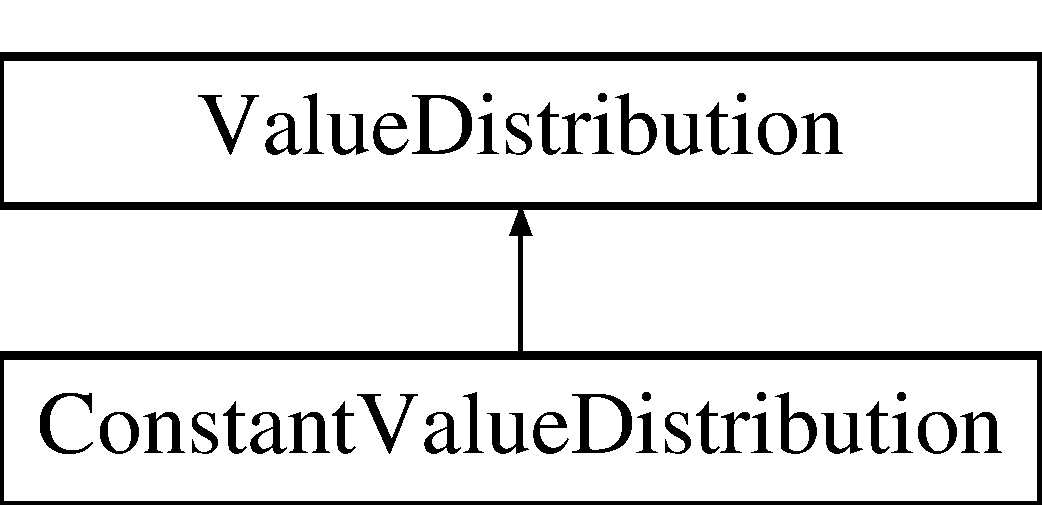
\includegraphics[height=2cm]{classValueDistribution}
\end{center}
\end{figure}
\subsection*{Public Member Functions}
\begin{DoxyCompactItemize}
\item 
\hypertarget{classValueDistribution_ad39dd4a07241d433bb8f5ac5026c1d6d}{
virtual string $\ast$ {\bfseries getNext} ()=0}
\label{classValueDistribution_ad39dd4a07241d433bb8f5ac5026c1d6d}

\end{DoxyCompactItemize}


\subsection{Detailed Description}
Abstract class representing the distribution of values to be written to the database 

The documentation for this class was generated from the following file:\begin{DoxyCompactItemize}
\item 
src/ValueDistribution.h\end{DoxyCompactItemize}

\printindex
\end{document}
